\documentclass[10pt,a4paper]{report}
\usepackage[utf8]{inputenc}
\usepackage{amsmath}
\usepackage{amsfonts}
\usepackage{amssymb}
\usepackage{a4wide} %Wider margins
\usepackage[english]{babel} %English dictionary for hyphenation and definitions, e.g. Table vs. Tabel
\usepackage[official]{eurosym} %Support for Euro-sign
\usepackage[utf8]{inputenc} %Support for internationalization, e.g. é vs.\’e
\usepackage{amsmath,amssymb,amsthm} %Support for mathematical formulas and symbols
\usepackage{fancyhdr} %Fancy headers
\usepackage{hyperref} %Creates clickable links
\usepackage{graphicx} %Support for grahpics
\usepackage{nopageno} %Support for removal of pagenumbers
\usepackage{tabularx}
\usepackage{enumitem}
\usepackage{xspace}
\usepackage{array}
\usepackage{algorithm,algpseudocode}
\usepackage{float}
\usepackage{mathtools}
\usepackage[table, xcdraw,dvipsnames]{xcolor}
\usepackage[titletoc,toc,title]{appendix}
\usepackage{listings}
\usepackage{pdfpages}
\usepackage{footmisc}
\usepackage{attachfile2}
\usepackage{subfig}
\usepackage{amsmath}
\usepackage{rotating}
\usepackage{algorithm}
\usepackage{multirow}
\usepackage{algpseudocode}
\usepackage{rotating}
\usepackage{import}
\usepackage{listings}
\usepackage{makecell}
\graphicspath{ {./ThesisFigures/} }

\hypersetup{
    pdftitle={}, %PDF-file will be given a proper title when viewed in a reader
    hidelinks %PDF-file will be given clickable, yet not visible links when viewed in a reader
}

\newcommand{\documenttitle}{A computational biology framework}
\newcommand{\documentsubtitle}{A data analysis tool to support biomedical engineers in their research}


\newcommand{\true}{{\sc True}\xspace}
\begin{document}

	
%	\begin{titlepage}
%		
%		\center
%		
%		\vspace*{3cm}
%		
%		\textbf{\huge \documenttitle} 
%		
%		\textit{\LARGE \documentsubtitle}
%		
%		\vspace*{2cm}
%		
%		\large
%		\centering
%		T.P.A.~\textsc{Beishuizen}~(0791613)\\
%		Email: \texttt{t.p.a.beishuizen@student.tue.nl} \\
%		1 October 2017 - 23 October 2018\\
%		Eindhoven University of Technology\\
%		
%		\vspace*{1cm}
%		
%		Biomedical Engineering - Computational Biology (8ZM104)\\
%		Exam committee: \\
%		Dr. Dragan Bo\v{s}na\v{c}ki (\texttt{d.bosnacki@tue.nl}) \\
%		Dr. Ir. Veronika Cheplygina (\texttt{v.cheplygina@tue.nl}) \\
%		Prof. Dr. Peter Hilbers (\texttt{p.a.j.hilbers@tue.nl}) \\
%		
%		\vspace*{1cm}
%				
%		Data Science and Engineering - Data Mining (2IMC00)\\
%		Exam committee: \\
%		Dr. Dragan Bo\v{s}na\v{c}ki (\texttt{d.bosnacki@tue.nl}) \\
%		Dr. George Fletcher (\texttt{g.h.l.fletcher@tue.nl}) \\
%		Dr. Ir. Joaquin Vanschoren (\texttt{j.vanschoren@tue.nl})
%		
%		
%		\vfill
%		
%		\vspace*{1cm}
%		
%		\today
%		
%	\end{titlepage}
	
%	\tableofcontents
	
	%\newpage
	
	\pagestyle{fancy}
	%Abbreviations used by fancyhdr:
	%E Even page
	%O Odd page
	%L Left field
	%C Center field
	%R Right field
	%H Header
	%F Footer
	\fancyhead{} % clear all header fields
	\fancyfoot{} % clear all footer fields
	\renewcommand{\headrulewidth}{0.4pt}
	\renewcommand{\footrulewidth}{0.4pt}
	
	\fancyhead[L]{\rightmark}
	\fancyfoot[C]{\thepage}
	\fancyhead[R]{T.P.A. Beishuizen}
	
	
	\clearpage
	
	\chapter{Automatic feature selection for high-dimensional biomedical data}
	\label{chap:FeatureSelection}
	
	\section{Introduction}
	\label{FSsec:Introduction}
	
	% Topic dimensionality reduction
	For a biomedical engineering framework dimensionality reduction is important.  Some biomedical datasets contain a high number of features, whereas only a selection of those features are interesting. A direct link of features to the output is desired, therefore especially dimensionality reduction based on feature selection is important. Multiple projects attempted to reduce the number of features \cite{baumgartner2006data, welthagen2005comprehensive} which resulted in multiple algorithm proposals \cite{lim2003planar, peng2010novel, biesiada2007feature, ding2005minimum} and tests on their performance \cite{catal2009investigating, liu2002comparative}. The research goal is \emph{to evaluate the performance of feature selection methods and make a choice on which methods should be added to the framework}. In this document several of those algorithms are presented and test their quality.
	\\
	
	% Introduction
	For this research one programming language is used, \textit{Python} version 3.6. This language was chosen, due to the numerous possibilities in preprocessing and analysis in the open source language \cite{mckinney2010data}. \textit{Python} makes use of packages containing additional classes and methods to be used in experiments. To easily import these packages the \textit{Anaconda} version 3 environment is used \cite{yan2018hands}. Packages available by \textit{Anaconda} and often used in the analyses are \textit{NumPy} \cite{walt2011NumPy}, \textit{SciPy} \cite{jones2014SciPy} and \textit{Scikit-learn} \cite{pedregosa2011scikit}. Aside from these widely used packages, the package \textit{TPOT} \cite{olson2016tpot} is used, as well.
	
	% To be added
	\textit{Dimensionality} \underline{TO BE ADDED}\\
	The dimensionality of a dataset in literature is the number of features of that dataset\cite{yu2003feature,lim2003planar,biesiada2007feature}. A high dimensionality therefore indicates a high number of features. The package \textit{metalearn} calls dimensionality the number of features divided by the number of instances. If this definition of dimensionality is used it is specifically stated. This definition is used to show possible imbalance between the number of features and instances and normally the dimensionality should be very low, at least $<1$.
	\\	
	% Introduction biomedical data
	\textit{Dataset issues} \underline{TO BE ADDED}
	The choice of a data analysis approach heavily depends on the nature of the data. The amount of data in the biomedical world is growing at an enormous rate, faster than biomedical engineers can analyse. Several additional challenges came up with this uncontrollable growth. These challenges are in many cases focused on data volume, dimensionality, complexity, heterogeneity and quality \cite{chen2006medical, doi:10.1093/bib/bbx044}.
	
	% Volume challenge
	Scientists tend to collect abundant data, which makes data sets bigger than needed. Both in number of instances and features, data sets are harder to understand or analyse when more instances and features are available \cite{chen2006medical}. This volume problem usually is tackled by taking sub-populations of the complete set. Sub-sets can either be focused around a part of the population (e.g. gender, age, race) or taken at random to still represent all of it. Due to the efficiency of analysis techniques and the rise in computational speed of servers \cite{blythe2008rise}, volume on its own becomes less of an issue. Volume does however become a challenge when it is combined with heterogeneity and quality \cite{Turkay2014, Holzinger2014}.
	
	% Dimensionality challenge
	Not all data sets have a high number of instances that causes a big data volume. Sometimes there are relatively few instances, while the number of features is disproportionally high \cite{dubitzky2007fundamentals}. This is also called high dimensionality (high number of features and low number of samples). Usually many of those features are not relevant enough for research, however are still used for testing. Trying to remove features that are not important significantly helps finding relations between the other features and create more knowledge about the research topic. Lowering the number of features also makes the data volume decrease, therefore making analysis easier. Essentially an optimal features set should be selected to obtain the best results \cite{PENG201015}.	
	
	\subsection{Data Symbols}  \underline{TO BE DISCUSSED - ONLY TABLE?}
	\label{subsec:DataSymbols}
	
	Often in this research project, equations and pseudo-algorithms are discussed. In these equations and pseudo-algorithms, several symbols were used to explain the data. A quick overview of these symbols is given (Table \ref{tab:DatasetSymbols}) as well as a more detailed description:
	
	\begin{itemize}
		\item \textit{$F$} -
		A list that contains all the names of the features. It is a list of size $m$ with $m$ being the number of features. A subset $x$ of $F$ is written as $F_x$.
		\item \textit{$S$} -  
		A list of all samples in a dataset. It is a list of size $n$ with $n$ being the number of samples. A subset $x$ of $S$ is named $S_x$ and a single sample is usually called $s$. 
		\item \textit{$X$} -
		A matrix that contains all sample values for every feature. It is an $n$ by $m$ matrix with $n$ being the number of samples and $m$ being the number of features. If the values of a specific feature $f$ or a subset of features $F_x$ are used this is written as $X_f$ and $X_{F_x}$ respectively, hence the column $f$ or columns $F_x$ are selected. Similarly for $X_s$ and $X_{S_x}$ the row $s$ or rows $S_x$ respectively are collected from $X$.
		\item \textit{$y$} -
		A vector that contains all class labels for every sample. It is a vector of size $n$ with $n$ being the number of samples.
		\item \textit{$W$} - 
		Weights given to a feature after training a feature selection technique. The weight of feature $f$ or set of features $F_x$ is called $W_f$ and $W_{F_x}$ respectively.
	\end{itemize}
	
	\begin{table}[]
		\caption{An overview of the symbols used to explain the data}
		\label{tab:DatasetSymbols}
		\begin{tabular}{|l|l|}
			\hline
			\textbf{Value} & \textbf{Description}                                   \\ \hline
			$m$				 & The number of features                                 \\ \hline
			$F$              & A list of ($m$) features                                 \\ \hline
			$n$				 & The number of samples                                 \\ \hline
			$S$              & A list of ($n$) samples                                  \\ \hline
			$X$              & A matrix of ($n \times m$) dataset values \\ \hline
			$y$              & A vector of ($n$) output labels                          \\ \hline
			$W$              & A list of feature weights                              \\ \hline
		\end{tabular}
	\end{table}
	
	\subsection{Related work}
	
	% Related work
	A good overview of all the techniques used can be found in a survey article \cite{saeys2007review} explaining all the algorithms used, as well as several others.
	Similar research has been done prior to this one. Numerous algorithms have been proposed for feature selection \cite{lim2003planar, peng2010novel, biesiada2007feature, ding2005minimum, donoho2008higher, SENAWI201747} and simple performance tests are done to do research on both these and other algorithms \cite{baumgartner2006data, catal2009investigating, liu2002comparative, CATAL20091040, huang2013automated}. Most of these focus on a much smaller number of features than in this research however, not testing the algorithms for data with more than 1000 features. Other feature selection research focus more on one type of the feature selection, being wrapper methods \cite{tsamardinos2017massively, el2009new, radovic2017minimum} or embedded methods \cite{jong2004feature}. 
	A select number of articles focused on bigger feature set sizes. One research looked at bigger not necessarily biomedical datasets and tried to use support vector machines for feature selection, one of these datasets also being the Arcene dataset \cite{chen2006combining}. A similar research focused on feature selection for a microarray dataset of 7000 and showed that feature selection is beneficial \cite{xing2001feature}. Another research looked at 35 datasets with a range of features between 37 and 50000 and what type of feature selection works best \cite{song2013fast}. They used five advanced algorithms and therefore harder to understand, whereas the ones used in our research are more intuitive. Another very similar research evaluated feature selection algorithms, too, but did not have the focus on the number of features.
	Much research is done on feature selection algorithms, as can be found in the related work. This work was made for using feature selection for biomedical data however, containing several benefits:
	\begin{itemize}
	\item	The main goal was to create a feature subset as small as possible with a performance as high as possible, which only rarely was a goal in other research \cite{prados2004mining}. This resulted in both a score being made that incorporates both the feature subset size and the performance as the FS\_score and the usage of this score to evaluate the usefulness of every feature. While not being a main goal, the computation time is also stored for additional investigations on that.
	\item	Feature selection is done on very big biomedical datasets of more than 1000 features, therefore the feature selection has a big influence. This is not often done, whereas these datasets will become more available as well as investigated in the future.
	\item	Only basic feature selection algorithms are used so other users can easily understand the basic principles and many different ones are investigated, making this work a very extensive search for well performing feature selection algorithms. Moreover, these algorithms are also very different in their feature selection, also showing the benefits and drawbacks of every type of algorithm.
	\item	At last automation of feature selection techniques is added, too. Automated machine learning is a very interesting approach to extracting information out of a dataset. Properly implementing feature selection in automated machine learning opens it up for high dimensional datasets, as well.
	\end{itemize}
	
	
	\section{Methods}
	\label{FSsec:Background}
	
	% Introduction background & layout background
	Before testing several feature selection methods, first the background of the study is explained. Firstly, the datasets and their characteristics are explained. Secondly, feature selection methods are discussed. Thirdly the concept automated machine learning is discussed as a possible technique to add to the framework, combined with a tool that implements automated machine learning.
	
	\subsection{Datasets}
	\label{FSsubsec:Datasets}
	
	% Data sets	
	Four datasets were used as a case study for the feature selection algorithms . Two sets are microarray datasets that are used for research on psoriasis \cite{nair2009genome, suarez2012expanding, bigler2013cross, yao2008type} and cancer \cite{wojnarski2010rsctc}. Two other sets are mass spectrometry data sets, used for research on cancer \cite{NIPS2004_2728} and micro organisms \cite{doi:10.1093/bioinformatics/btu022}. These four datasets all have a high number of features varying from 1300 to 54675 features with a number of samples varying from 200 to 580 samples (Table \ref{tab:DataSetDescriptions}). All of these datasets are based on classification as tests are done for different test subject groups, therefore the focus on feature selection algorithms will also be based on classification. Many features are expected to be irrelevant in this classification and therefore could be removed with feature selection.	

	\begin{table}[]
		\centering
		\caption{A schematic overview of the four datasets.}
		\label{tab:DataSetDescriptions}
		\begin{tabular}{ll|llll}
			\textbf{Dataset focus} & \textbf{Data type}                                          & \textbf{Features} & \textbf{Samples} & \textbf{Classes} & \textbf{Remarks}                                                                                                        \\ \hline
			Psoriasis        & Micro-array                                                 & 54675             & 580              & 3                & \begin{tabular}[c]{@{}l@{}}- Derived from five \\ different datasets \cite{nair2009genome, suarez2012expanding, bigler2013cross, yao2008type} \\ -- \end{tabular}                                       \\
			Cancer           & Micro-array                                                 & 54675             & 383              & 9                & \begin{tabular}[c]{@{}l@{}}- Used in a data \\ mining challenge \cite{wojnarski2010rsctc}\end{tabular}                                            \\ \hline
			Cancer           & \begin{tabular}[c]{@{}l@{}}Mass\\ Spectrometry\end{tabular} & 10000             & 200              & 2                & \begin{tabular}[c]{@{}l@{}}- Created for the \\ NIPS conference \cite{NIPS2004_2728}\\ - Several probe \\ features are present \\ -- \end{tabular} \\
			Micro-organisms  & \begin{tabular}[c]{@{}l@{}}Mass\\ Spectrometry\end{tabular} & 1300              & 571              & 20               & \begin{tabular}[c]{@{}l@{}}- Originates from a \\ micro organisms study \cite{doi:10.1093/bioinformatics/btu022}\end{tabular}                                                                                                                       
		\end{tabular}
	\end{table}

	\subsubsection{Micro-array Datasets} \underline{TO BE ADDED, ONLY GENERAL MENTIONS?}
	\label{PLsubsec:Microarray}
	
	% Introduction
	Micro-array data is a fairly new type of biomedical data. Datasets of this kind have information on expression levels of a high number of genes \cite{brazma2001minimum}. These expression levels can be used for gene level research, such as genome mapping, transcription factor activity and pathogen identifications. The data is gathered by fixing DNA molecules on a glass slide on specific spots. The nucleotide base pairs of those fixed DNA molecules can form hydrogen bonds with RNA corresponding to genes, testing the expression of those genes by how many bonds are made \cite{selvaraj2011microarray}.
	
	% Challenges
	Micro-array data is known to present challenges in data quality and needs normalisation for the data to be useful \cite{selvaraj2011microarray}. The thousands of features that are based in the data also indicate that feature selection is very important, so the irrelevant genes can be removed. Aside from that, size may also be an issue. Due to the sheer size of the data not all analyses will perform optimally in both time and quality. In this research two microarray datasets are used for research:
	
	\begin{itemize}
		% Psoriasis
		\item \textit{Psoriasis microarray dataset} \\ This dataset is comprised of five different data sets \cite{nair2009genome, suarez2012expanding, bigler2013cross, yao2008type}. These five different datasets consist of 54675 features, all corresponding to gene expression. Samples were collected from three different test subject groups: affected skin from test subjects suffering from psoriasis (214 samples), unaffected skin from test subjects suffering from psoriasis (209 samples) and skin from healthy test subjects (85 samples). Combining these three sample types gives 508 samples. Since the data comes from five different experiments, the data is normalized for every experiment.
		% Cancer
		\item \textit{Arcene: Cancer microarray dataset} \\ This dataset, called Arcene dataset, is used in a challenge focussing on classification problems with a low number of samples, but a high number of features \cite{wojnarski2010rsctc}. It consists of the same number of features as the Psoriasis data set, 54675 features corresponding to gene expression. It also has 383 samples corresponding to nine different test subject groups. The challenge did not provide labels for the test subject groups. Also these groups differ in size, one group corresponding to 150 samples and the others varying from 16 to 47 samples.
	\end{itemize}
	
	\subsubsection{Mass Spectrometry Datasets} \underline{TO BE ADDED, ONLY GENERAL MENTIONS?}
	\label{PLsubsec:MassSpect}
	
	Mass spectrometry data contains information on proteins and peptides \cite{cottrell1999probability, dettmer2007mass}. Analysis of this information is used in studies about proteins, also known as proteomics \cite{matthiesen2008analysis}. Mass spectrometry is a technique that can be used to find how much of a certain protein is present. This is done by measuring the mass of gas-phase ions originating from molecules of that protein, showing that protein is present. On top of that it can also measure the quantity of the mass, therefore showing how much of a protein is present \cite{watson2007introduction}.
	
	
	% Challenges
	Challenges in the analysis of mass spectrometry datasets are mainly found in the way this data is produced. The expression is given for several proteins and this expression can differ significantly between proteins. Therefore some type of normalisation is useful. Aside from that, in this technique usually a high number of proteins is tested at the same time. Therefore feature selection can be helpful to remove irrelevant genes. Two mass spectrometry datasets were used in this research:
	
	\begin{itemize}
		\item \textit{RSCTC: Cancer mass spectrometry dataset} \\ This dataset, called RSCTC dataset, was created as a classification problem to distinguish cancer patterns from normal patterns \cite{NIPS2004_2728}. It is created for the 'Neural Information Processing Systems' conference by merging three mass spectrometry datasets. It consists of 10000 features corresponding to either spectra of the mass spectrometry or probe variables without any predictive power. Samples from two groups are taken, from patients with ovarian or prostate cancer and from control patients. No labels are given to the groups, however it is known that one of the groups has 88 samples and the other 112 samples, combined in a total of 200 samples.
		% MicroOrganisms
		\item \textit{Micro organisms mass spectrometry dataset} \\ This dataset is created to back up a proposed method for routinely performing direct mass spectrometry based bacterial species identification \cite{doi:10.1093/bioinformatics/btu022}. It consists of 1300 features corresponding to different spectra of the mass spectrometry data and 20 test subject groups corresponding to Gram positive and negative bacterial species. Gram classification is a result of a Gram stain test \cite{madigan2017brock}. The groups differ in size varying from 11 to 60 samples, making a total of 571 samples.
	\end{itemize}
	
	\subsection{Feature Selection Methods}
	\label{FSsubsec:FeatureSelectionMethods}
	
	% Introduction feature selection
	Feature selection is a way to perform dimensionality reduction. In feature selection a subset of features is chosen to represent the complete sample space \cite{Guyon2006}. Several techniques are available to choose a representation subset and the effectiveness of these techniques has been tested multiple times \cite{CATAL20091040, molina2002feature}. These techniques can be grouped accordingly in three different categories: \textit{filter methods}, \textit{wrapper methods} and \textit{embedded methods} \cite{saeys2007review}. Each of these methods is explained in what follows. For better understanding of the different feature selection methods, pseudo-algorithms are created for each of them.

	\subsubsection{Filter Methods}
	\label{FSsubsec:FilterMethods}
	
	% Introduction filter methods
	Filter methods are based on giving relative ranks to the features in a feature space. All features are given a value based on their performance and are ranked by those values \cite{Duch2006, saeys2007review}. Several methods are used to rank the features. These methods are usually based on splitting data matrix $X$ twice. First they are split by feature ($X_{f_1}, X_{f_2} ... X_{f_n}$) for computation. Secondly the columns are split by output classes $c_1, c_2 ... c_n$ ($X_{f}^{c_1}, X_{f}^{c_2} ... X_{f}^{c_p}$) to distinguish the predictive power for features between classes. A ranking method would quantify the significance according to these values. This results in ranking method $R(X_f, y)$ in which sample label $y$ is used to split the data per class. For illustration a ranking method collection is given:
	
	\begin{itemize}
		% T-test binary
		\item \textit{T-test and ANOVA} \\ 
		Statistics can be used to compare groups with each other. In statistics these groups are seen as separate distributions, which may or may not be seen as independent distributions. If there are two groups  a t-test can be done to find the chance for these groups to originate from the same distribution\cite{heiberger2004statistical}. 
		For sample classifications the groups would consist of samples with the same label ($X_{f}^{c_1}$  and $X_{f}^{c_2}$). For example, the t-test can be done between group with class $c_1$ and group with class $c_2$. If the values of a certain feature from these groups are highly unlikely to follow the same distribution ($R(X_{f}^{c_1}, X_{f}^{c_2})$), the p-value will be very low and therefore the rank will be higher.
		
		If there are more than two groups that must be checked whether they are from the same distribution ($R(X_{f}^{c_1}, X_{f}^{c_2} ... X_{f}^{c_p})$), a t-test cannot be used. In this case the option is available for a multiple group testing, also called analysis of variance (ANOVA). ANOVA computes whether not only two, but multiple groups can originate from the same distribution. ANOVA needs equal group sizes, otherwise the results of the tests are less reliable. The less powerful Kruskall Wallis test can be used if this reliability is needed. Another disadvantage is that t-test and ANOVA should only be used if the groups follow a normal distribution, which might not be the case \cite{heiberger2004statistical}.
		
		% Mutual information
		\item \textit{Mutual information} \\
		Mutual information is another way of matching features with the results. The relevance of using one variable to predict the other variable is used in the equation to compute mutual information. 
		
		\textit{Mutual information \underline{TO BE COMBINED}} \\
		Mutual information can be used on two different variables. The relevance of using one variable to predict the other variable is used in the equation to compute mutual information (Equation \ref{eq:MutualInformation}). In this equation the probability density function $p$ is used to find the mutual information (MI) between variables $x$ and $y$ \cite{peng2005feature}. Mutual information can be used for both classification and regression. It was initially meant for use in communication channels, however its statistical decision making capabilities made it a good filter method \cite{battiti1994using}.
		
		\begin{equation}\label{eq:MutualInformation}
		MI(x, y) = \sum_x \sum_y p(x, y) \log{\frac{p(x, y)}{p(x)p(y)}}
		\end{equation}
		
	\end{itemize}
	
	% Feature selection threshold criteria
	These ranking methods $R$ to rank the features are only the first step in the filter methods. The next step is choose which features to filter out based on $R$. A quick approach would be to choose a number or fraction $n$ and select the top $n$ ranked features from the complete space (Algorithm \ref{alg:FilterTopNAlgorithm}). Another approach would be to use thresholds derived from literature \cite{donoho2008higher}. For the t-test, a p-value of $0.05$ is often chosen as the threshold value \cite{storey2003statistical, higgins2003measuring}.
	
	\begin{algorithm}[H]
		\caption{A basic top $n$ filter algorithm \cite{Duch2006}}\label{alg:FilterTopNAlgorithm}
		\begin{algorithmic}[1]
			\Procedure{FilterSelection($X, y, F, R, n$)}{}
			\State $F_{\textit{selected}} \gets \O$ 	\Comment{Start with empty feature set}
			\State $Z \gets \O$							\Comment{Start with empty set of ranking values}
			\For {$f \textbf{ in } F$} 					\Comment{For all features in $F$}
			\State $Z_f \gets R(X_f, y)$ 				\Comment{Compute the ranking value between feature and output} 			
			\State $Z \gets Z \cup \{Z_f\}$ 				\Comment{Add the ranking value to the set of ranking values}
			\EndFor
			\State $\textbf{Sort } F \textbf{ by } Z$ \Comment{Sort the features by their ranking value}
			\State $F_{}selected \gets F_{[1,n]}$ \Comment{Select the top n features from the sorted feature set}
			\State $\textbf{return } F_{\textit{selected}}$
			\EndProcedure
		\end{algorithmic}
	\end{algorithm}	

	
	% Advantages, disadvantages filter methods	
	Using filter methods has its advantages and disadvantages. These filter methods are very computationally efficient. Every feature is given a value for its rank and then a subset is selected based on those ranks. These filter methods however do not take into account dependencies between features. These dependencies could make the final feature subset worse, as maybe some features are related. Other methods are better at handling those dependencies \cite{Duch2006, saeys2007review}.
	
	\subsubsection{Wrapper Methods}
	\label{FSsubsec:WrapperMethods}
	
	% Introduction wrapper methods
	Filter methods take into account the direct relation between features and the output classes, whereas wrapper methods focus more on the subsets of features and their ability to classify the data. Wrapper methods try to find the best combination of features to classify the given data and take into account the change when adding or removing features from a candidate subset. The choice of subset selection is "wrapped"  around the quality computation, therefore this method is called a wrapper method \cite{Reunanen2006}. Since an exhaustive search of trying out all possible subsets would span a computation time of $2^n$ with $n$ being the number of features \cite{Alsallakh2016PowerSet}. This combinatorial explosion should be avoided and therefore less computationally intensive approximation concepts have been constructed. Three of those concepts are explained, focusing on basic sequential search, extensions of sequential search and stochastic search.
	
	% Evaluation method
	Before explaining the possible wrapper methods, first the evaluation function $J$ should be discussed. To find out which subset of features can classify the data the best way, a function should be used to evaluate the performance of the subset \cite{Reunanen2006}. Evaluation functions can be based on conditional independence \cite{Reunanen2006,tsamardinos2017massively}, showing the difference in performance for a subset with and without a certain feature. Other evaluation functions are based on machine learning techniques \cite{huang2013automated, saeys2007review}, rating the ability to classify the outcome. Several interesting approaches for evaluation functions are shown in maximum relevance, minimum redundancy algorithms \cite{SENAWI201747, el2009new, radovic2017minimum} (MRMR algorithms). In these MRMR algorithms, several different evaluation functions are used based on the ability of features to classify the outcome (relevance) and the presence of correlation between features (redundancy). In this project, the evaluation function is fixed on the machine learning algorithm Naive Bayes, due to its understandability.
	
	\begin{itemize}
		% Sequential search
		\item \textit{Sequential search} \\
		The first concept to be explained is sequential search. This wrapper method tries to improve a candidate subset by evaluating the change of the sequential addition or removal of a specific feature. Therefore, two types of sequential search are possible, known as forward selection and backward selection. Forward selection starts with the empty subset. Every feature is iteratively evaluated and added to the feature subset if the evaluation function shows an increase in prediction. A maximum feature subset selection size $l$ can be defined if needed, as well. The layout of forward selection is shown as a pseudo algorithm (Algorithm \ref{alg:ForwardSelection}) for understanding \cite{Reunanen2006}.
		
		% Backward selection
		Backward selection does the opposite of forward selection. It starts with the complete feature set in which every feature is iteratively evaluated by the evaluation function for its contribution. If the evaluation function shows that its contribution is very small, it is removed. This way only features with a high impact will remain in the subset. The maximum number features that can be removed $r$ can be defined if needed, as well. be A layout of backward selection is shown as a pseudo algorithm (Algorithm \ref{alg:BackwardSelection}) for understanding, as well \cite{Reunanen2006}.
		
		% Order discussion
		In both forward and backward selection the sequence order is important. Different feature subsets will be made for different order of features. The ordering can be changed in a specific way if needed. Examples would be using the ranking concepts used by filter methods. Another possibility would be to randomize the order and run the algorithm multiple times to find the best subset \cite{Reunanen2006}.
		
		% Insert pseudo-algorithm for forward and backward sequential search
		\begin{algorithm}[H]
			\caption{A forward selection sequential search algorithm \cite{Reunanen2006}}\label{alg:ForwardSelection}
			\begin{algorithmic}[1]
				\Procedure{SequentialForwardSelection($X, y, F, J, \alpha, l$)}{}
				\State $F_{\textit{selected}} \gets \O$				\Comment{Start with empty feature set selection}
				\For {$f \textbf{ in } F$}							\Comment{For all features in $F$}
				\If {$J(X_{F_\textit{selected}}, y, X_f) > \alpha$}	\Comment{Check if evaluation is higher than $\alpha$ with feature $f$}
				\State $F_{\textit{selected}} \gets F_{\textit{selected}} \cup \{f\}$	\Comment{Add $f$ to the feature set selection}
				\EndIf
				\If {$\text{length}(F_{\textit{selected}}) = l$}	\Comment{Stop if size of feature set selection has been reached}	
				\State $\textbf{break}$
				\EndIf
				\EndFor
				\State $\textbf{return } F_{\textit{selected}}$
				\EndProcedure
			\end{algorithmic}
		\end{algorithm}
		
		\begin{algorithm}[H]
			\caption{A backward selection sequential search algorithm \cite{Reunanen2006}}\label{alg:BackwardSelection}
			\begin{algorithmic}[1]
				\Procedure{SequentialBackwardSelection($X, y, F, J, \alpha, r$)}{}
				\State $F_{\textit{selected}} \gets F$				\Comment{Start with complete feature set selection}
				\For {$f \textbf{ in } F_{\textit{selected}}$}		\Comment{For all features in $F_{\textit{selected}}$}
				\If {$J(X_{F_{\textit{selected}} \backslash \{f\}} , y, f) < \alpha$} \Comment{Check if evaluation is higher than $\alpha$ without $f$}
				\State $F_{\textit{selected}} \gets F_{\textit{selected}} \backslash \{f\}$ \Comment{Remove $f$ from the feature set selection}
				\EndIf
				\If {$\text{length}(F \backslash F_{\textit{selected}}) = r$} \Comment{Stop if feature removal limit has been reached}
				\State $\textbf{break}$
				\EndIf
				\EndFor
				\State $\textbf{return } F_{\textit{selected}}$
				\EndProcedure
			\end{algorithmic}
		\end{algorithm}
		
		% Extension sequential search
		\item \textit{Sequential search extension} \\
		The two basic sequential search algorithms forward and backward selection can be altered for better use. An intuitive idea would be to combine the two algorithms, creating an algorithm that first selects features with the evaluation function followed by removing them according to the evaluation function or the other way around. Also there is no restriction on only doing one iteration of both forward and backward selection, giving rise to "plus l-take away r" selection (PTA). $\text{PTA}(l, r)$ adds $l$ features with forward selection and removes $r$ features with backward selection per iteration, eventually converging to an optimum. 
		These found optima in both sequential search algorithms and possible extensions can converge to local optima. Beam search is an example that also collects suboptimal branches for possible better optima, instead of only keeping the best possible outcome at all times \cite{Reunanen2006}.
		
		A last example of a sequential search extension is called floating search. Instead of adding and removing a set number of features as in PTA, floating search continues to add and remove features until the best subset is found, doing a forward and backward search iteratively. Since feature relevance and redundancy changes for every new subset, all features are continuously evaluated to find out if they must be added to or removed from the subset. This way an optimal subset can be found \cite{Reunanen2006}.
	\end{itemize}
	
	% Advantages/Disadvantages
	The major advantage of using wrapper methods is that they also take into account possible dependencies between features. The computation time of wrapper methods usually is higher than of filter methods, but still relatively short as it should always converge to an optimum. These optima can be local however, so the result may not be the optimal, due to its greedy character. Also, these methods are dependent on the evaluation function and are known to be prone for over fitting \cite{Reunanen2006, saeys2007review}.
	
	\subsubsection{Embedded Methods}
	\label{FSsubsec:EmbeddedMethods}
	
	% Introduction Embedded methods
	In both filter and wrapper methods, machine learning plays little to no role in selecting features. Filter methods do not use learning at all and a wrapper method can only use machine learning for evaluating feature subsets. Several machine learning algorithms contain attributes that can be used directly to select or eliminate features from the ideal feature set selection, for example the coefficients in linear SVM. Embedded methods combine feature selection with a machine learning algorithm $M$, in contrast to wrapper methods in which these are separated \cite{Lal2006}. Usually this combination involves using the weights given to features by machine learning algorithms \cite{blum1997selection}.
	
	One approach to solve feature selection is based on contribution relaxation minimization. Since the theoretical approach of embedded methods can be very computationally intensive an approximation of the minimization problem is given, showing an example embedded method \cite{Lal2006}.
	
	
	\begin{itemize}
		\item \textit{Contribution relaxation minimization} \\
		
		% Explanation contribution relaxation
		Contribution relaxation is based on giving every feature $f$ a contribution factor $\sigma_f \in [0, 1]$. This contribution factor shows the contribution of a feature to the preferred outcome. The final goal is to select a subset of features, though, and not use all features with a contribution factor. To achieve that a minimization function is used in which all contribution factors become $\sigma_f \in \{0, 1\}$. With contribution factors in $\{0, 1\}$, a subset with all features having $\sigma_f = 1$ can be selected as the ideal subset \cite{Lal2006}. 
		
		% Approximation of methods
		The minimization can be implemented with an embedded method. This method would however be computationally intensive and therefore approximations are used. The most used approximation is similar to the filter methods, ranking each feature and choosing features based on rank (Algorithm \ref{alg:EmbeddedForwardSelectionAlgorithm}). This embedded method is also called a forward selection method. A machine learning algorithm $M$ assigns a weight to each feature, which can be used as a rank (Algorithm \ref{alg:FilterAlgorithm}). The difference between a ranking method $R$ of the filter methods and the weights of a machine learning algorithm $M$ is that $M$ also takes into account the dependency between features \cite{Lal2006}.
		
		\begin{algorithm}[H]
			\caption{An embedded forward selection algorithm \cite{Lal2006}}\label{alg:EmbeddedForwardSelectionAlgorithm}
			\begin{algorithmic}[1]
				\Procedure{EmbeddedForwardSelection($X, y, F, M, \alpha$)}{}
				\State $F_{\textit{selected}} \gets \O$ 	\Comment{Start with empty feature set}
				\State $W \gets M(X, y)$					\Comment{Extract the weights for every feature}
				\For {$f \textbf{ in } F$} 					\Comment{For all features in $F$}
				\If {$W_f > \alpha$}			\Comment{Check if weight is higher than threshold $\alpha$}
				\State $F_{\textit{selected}} \gets F_{\textit{selected}} \cup \{f\}$ \Comment{Add $f$ to selected features}
				\EndIf
				\EndFor
				\State $\textbf{return } F_{\textit{selected}}$
				\EndProcedure
			\end{algorithmic}
		\end{algorithm}
	\end{itemize}
	
	% Examples of weights
	The weights given by machine learning are different for every algorithm. A first and most obvious example of an algorithm giving weights are algorithms based on linear support vector machines (linear SVM, from now on called SVM). The coefficients given by SVM give the features a contribution factor in the outcome \cite{jong2004feature, prados2004mining, zhang2006recursive, guyon2002gene}. A second example would be using decision trees and random forests. Decision trees use features to reduce the entropy between a set by splitting it in two subsets with a threshold and a feature. These splitting features can be used as a subset to create an effective feature selection outcome \cite{geurts2005proteomic, wu2003comparison, Duch2006}. To overcome an over fitting problem, commonly occurring in decision trees, random forests can be used instead and the best splitting features can be used \cite{liaw2002classification}.
	
	
	\subsubsection{Tree-based Pipeline Optimization Tool} \underline{TO DO: Add automated machine learning and meta-learning paragraphs and simplification}
	\label{FSsubsec:TPOT}
	
	% Introduction TPOT
	Tree-based Pipeline Optimization Tool (TPOT) is a tool that implements autoML. It uses machine learning pipelines and genetic programming to find the best solution for every data set. TPOT makes use of this genetic programming with using the machine learning pipelines in a tree. \textit{TPOT} consists of preprocessing and machine learning algorithms, that form the backbone of the pipelines. Their hyper-parameters are the variables. \textit{TPOT} makes mostly use of the machine learning and preprocessing algorithms of \textit{scikit-learn} from \textit{Python} in which it is also written, but also several additional algorithms are present (e.g. a hot encoding algorithm).
	
	% Biomedical preprocessing
	Considering the capabilities from \textit{TPOT} to cope with challenges in biomedical data, several methods are available. It has several different normalisation/standardisation scalers (StandardScaler, RobustScaler, MinMaxScaler) to tackle feature heterogeneity between different data sets and errors. It also has some feature selection operators to tackle errors (VarianceThreshold, SelectKBest, SelectPercentile). Wrapper methods however are not included, which may perform better in some situations. At last, if missing values are present, it imputes the median for those values before starting the evolutionary algorithm. However, it does not have any possibilities to handle non-numeric data. If non-numeric data is present, the user first needs to preprocess himself.
	
	% Disadvantage
	A big variety of algorithms are present for TPOT, as well as numerous hyper parameter values for those algorithms. This is both an advantage as an disadvantage as probably most algorithms and hyper parameter combinations are not useful as an outcome. Since TPOT randomly chooses mutations, possibly better algorithms could be chosen with less random choices. For example meta-features could be used to improve the algorithm selection.

	\section{Methods}
	\label{FSsec:Methods}
	
	% Introduction methods
	For empirical evaluation the collection of feature selection methods experiments are done. The quality of the feature selection is tested by defining a definition of quality first. After that an exploration of feature selection is done with filter methods, followed by comparisons of multiple feature selection methods. The four example datasets (subsection \ref{DEsubsec:Datasets}) were used as example datasets for the experiments.
	
	\subsection{Feature Selection Quality}
	\label{FSsubsec:DimensionalityReductionQuality}
	
	% Machine learning for testing
	To find out the quality of the feature selection, multiple machine learning algorithms are used \cite{hall1998practical}.  Classification of the datasets can be done with several machine learning algorithms and validation and tests scores show how well the data can be classified after feature selection. The quality will be described with the accuracy of machine learning algorithms: the number of right classifications divided by the total number of classifications. Five different machine learning classifiers are used from \textit{scikit-learn}: logistic regression, decision trees, nearest neighbour, support vector machines and Naive Bayes. Better feature selection algorithms have relatively higher accuracy, as they are better at preserving the right features. Since over fitting sometimes happens when fitting data in a machine learning algorithm, both a validation and a test score is computed for the accuracy. For every experiment a training set and a test set is created, making the test set 20\% of the complete dataset. A validation score is computed by using the "leave one out" technique on the training set and a test score is computed by testing the classification score of the test set. Since the samples are not evenly distributed over the classes the precision, recall and F1 scores are also computed to find potential bias in the result.
	
	% Addition to number of features
	In some cases the quality of the machine learning algorithm lacks a factor of feature subset size. The standard score in those cases is not sufficient enough to evaluate the result. To incorporate the quality of feature selection a new modified quality term \textit{FS\_score} is created (Equation \ref{eq:FSAccuracy}). In \textit{FS\_score} a modified version of the original score, in this thesis being accuracy, is given by first multiplying it by a factor dependent on the number of features. This factor consists of a constant $\beta$, a value in range $[0, 1]$ which can be chosen for the influence of the  value that represent the number of features. In practice $\beta > 0.95$ so the reduction does not have too much influence on the score.
	
	\begin{equation*}
	\label{eq:FSAccuracy}
	\text{FS\_score} = \text{score} \times \beta^{\text{\#features}}
	\end{equation*}
	
	% Absolute number of features
	The factor \mbox{\#features} is an absolute count, instead of a relative count (for example a percentage of features). The reason for using an absolute count can be found in the goal of the data analysis. In data analysis the number of features that can be relevant are very limited. Useful results need relations between the input and the output, and these relations need to be as simple as possible. If the number of features is relative to the total number of features, the input size can change significantly. Take for example the Micro-organisms and the RSCTC datasets provided for this stud. 2\% of the total features would be 26 and 1100 features for these datasets respectively. Whereas relations between 26 features and the output is possible to understand, relations between 1100 features and the output is much harder. Taking an absolute number of features allows for a more active choice on the input size.
	
	% Selection proper beta
	To put the impact of the \textit{FS\_score} in perspective, an example figure is made how the outcome is computed (Figure \ref{fig:FSAccuracyExample}). This figure shows the impact on the performance of a method when using a certain number of features. After using a correction factor, an optimum is created for which the number of features is important, the old optimal score did not include the number of features. The example (with $\beta = 0.99$) seems to give a good indication of the desired outcome. For every $10$ features, the \textit{FS\_score} is reduced by about 10\%, which meant for the example filter method that for 50 features an optimum was reached (Figure \ref{fig:FSAccuracyExample}). Because of this empirically found desired trade-off, $\beta = 0.99$ will be chosen in this project when using \textit{FS\_score}. 
	
	% Insert figures
	\begin{figure}[H]
		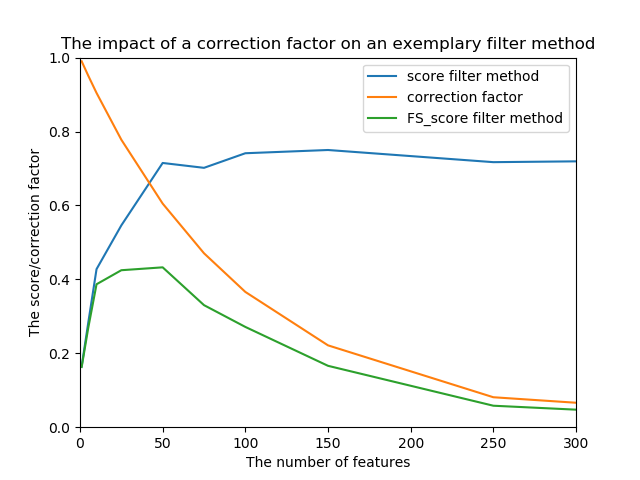
\includegraphics[]{FS_accuracy_example.png}
		\caption{An example of the impact of the correction factor on the score, in this case accuracy. The shown correction factor uses $\beta = 0.99$. On the x-axis the number of features is shown and on the y-axis the value for the original accuracy, the correction factor and the \textit{FS\_score}.}
		\label{fig:FSAccuracyExample}
	\end{figure}
	
	\subsection{Feature Selection Exploration}
	\label{FSsubsec:FeatureSelectionExploration}
	
	% First experiment
	The first set of experiments is used to explore a combination of the basic filter method combined with the quality measurements. The basic filter method algorithm selecting the top $n$ features (Algorithm \ref{alg:FilterTopNAlgorithm}) is used. The changing variables are the dataset, the ranking method, the feature preservation values and the accuracy computation methods (Table \ref{tab:FirstExperimentRequirements}). The range of chosen feature preservation values comes from both its ability to show impact of separate features (more impact from fewer features) and the relevance of keeping that number of features (irrelevant feature selection when having more than 1000 features). All of this together results in a total of $4 (\text{datasets}) \times 2 (\text{ranking methods}) \times 11 (\text{top } n \text{ features}) \times 5 (\text{accuracy computation methods}) = 440$ experiments. These experiments are visualized in eight plots, one plot for every combination of data set and ranking method. These plots then show the change in quality for different number of preserved features.
	
	\begin{table}[]
		\centering
		\caption{The four meta-parameters with their possible values in the first experiment.}
		\label{tab:FirstExperimentRequirements}
		\begin{tabular}{l|ll}
			\textbf{Variable} & \textbf{Description}                                                                              & \textbf{Values}                                                                                                                         \\ \hline
			Dataset           & The datasets used (subsection \ref{FSsubsec:Datasets})                                                                                 & \begin{tabular}[c]{@{}l@{}}Psoriasis\\ RSCTC\\ Arcene\\ Micro-Organisms\\ --\end{tabular}                                               \\
			Ranking method    & \begin{tabular}[c]{@{}l@{}}The method used for ranking \\ the features (
				Subsection \ref{FSsubsec:FilterMethods})\end{tabular}               & \begin{tabular}[c]{@{}l@{}}T-test (\textit{SciPy})\\ Mutual Information (\textit{scikit-learn})\\ --\end{tabular}                                                                \\
			Feature preservation values & \begin{tabular}[c]{@{}l@{}}The fixed size of the feature subset \\ after feature selection\end{tabular} & \begin{tabular}[c]{@{}l@{}}1, 5, 10, 25, 50, 75, \\ 100, 150, 250, 500, 1000\\ --\end{tabular}                                          \\
			F1-score computation & \begin{tabular}[c]{@{}l@{}}The machine learning algorithms \\ used to compute the F1-score (subsection \ref{FSsubsec:DimensionalityReductionQuality})\end{tabular}   & \begin{tabular}[c]{@{}l@{}}Naive Bayes\\ Logistic Regression\\ Support Vector Machine\\ Decision Tree\\ Nearest Neighbours\end{tabular}
		\end{tabular}
	\end{table}
	
	\subsection{Feature Selection Algorithms Evaluation}
	\label{FSsubsec:FeatureSelectionAlgorithmsEvaluation}
	
	% Second experiment
	The second set of experiments compares the feature selection methods in both feature selection and quality. For this experiment the four datasets are used with the logistic regression quality measurement, since the logistic regression gave the most consistent result of the five machine learning algorithms, showing the smallest variation across the datasets. The average performance for all datasets is also computed for clarification purposes. An overview of feature selection methods is made (Table \ref{tab:SecondExperimentMethods}) and all separate meta-parameters are explained here.
	Spectra are made with the results of the experiment that show the performance of all different combinations, showing the accuracy, precision, recall and F1-score. On top of that the computation time is computed and shown per algorithm, as well, in a separate bar chart. At last a combination of the earlier proposed \textit{FS\_score} and the computation time is shown as well for $\alpha = 0.99$ to show the relation between computation time on one hand and the \textit{FS\_score} on the other hand. 
	Several discussed algorithms  are chosen to be excluded from the evaluation. This choice is based on their poor scalability with regards to computation time and therefore unfit for datasets with this many features. These excluded algorithms are the backwards elimination sequential method, the simulated annealing stochastic search method and the embedded backwards elimination method (Subsection \ref{FSsubsec:FeatureSelectionMethods}). 
	
	\begin{table}[]
		\centering
		\caption{The methods that are evaluated in the second experiment setup.}
		\label{tab:SecondExperimentMethods}
		\begin{tabular}{l|ll}
			\textbf{Type}                    & \textbf{Method}                                                             & \textbf{Parameters}                                                                                                                                                                          \\ \hline
			Filter methods                   & \begin{tabular}[c]{@{}l@{}}Basic Filter Methods\\ (Algorithm \ref{alg:FilterTopNAlgorithm})\end{tabular} & \begin{tabular}[c]{@{}l@{}}- Rank: T-test, Mutual Information\\ - Thresholds: 50, 100, 150 features\end{tabular}                                                                             \\ \hline
			\multirow{3}{*}{Wrapper methods} & \begin{tabular}[c]{@{}l@{}}Forward selection\\ (Algorithm \ref{alg:ForwardSelection})\end{tabular}    & \begin{tabular}[c]{@{}l@{}}- Order: Random, Mutual Information\\ - Evaluation: Naive Bayes\\ - Alpha: 0.01, 0.001\\ --\end{tabular}                                             \\
			& \begin{tabular}[c]{@{}l@{}}PTA\\ (Algorithm \ref{alg:PTA})\end{tabular}                  & \begin{tabular}[c]{@{}l@{}}- Order: Random, Mutual Information\\ - Evaluation: Naive Bayes\\ - {[}l, r{]} = {[}20, 10{]}, {[}5, 2{]}\\ - Alpha: 0.01, 0.001\\ --\end{tabular} \\
			& \begin{tabular}[c]{@{}l@{}}Floating search\\ (Algorithm \ref{alg:FloatingSearch})\end{tabular}      & \begin{tabular}[c]{@{}l@{}}- Order: Random, Mutual Information\\ - Evaluation: Naive Bayes\\ - Alpha: 0.01, 0.001\end{tabular}                                                                                 \\ \hline 
			Embedded methods                 & \begin{tabular}[c]{@{}l@{}}Forward selection\\ (Algorithm \ref{alg:EmbeddedForwardSelectionAlgorithm})\end{tabular}    & \begin{tabular}[c]{@{}l@{}}- Machine Learning: SVM, RandomForests\\ - Threshold: 50, 100, 150 features\end{tabular}                                                                         
		\end{tabular}
	\end{table}
	
	\subsection{TPOT Feature selection integration}
	\label{FSsubsec:TPOTEvaluationIntegration}
	
	% Introduction
	TPOT is an effective tool to find the best machine learning pipeline for a certain dataset. Two restrictions hinder optimization regarding feature selection:
	
	\begin{enumerate}
		\item \textit{Lack of warm start} \\
		TPOT has a vast array of machine learning and preprocessing algorithms to find the best possible pipeline. Due to the number of possibilities being very high, a lot of time may be wasted due to searching in wrong directions. For feature selection, a pre-defined selection of pipelines (also known as a warm start) would improve efficiency.
		\item \textit{Feature selection possibilities} \\
		Several filter and embedded methods are present (Subsection \ref{FSsubsec:FeatureSelectionMethods}). All of these select percentages of feature selection, though. Still a high number of features can be present in the result after using percentages. On top of that, no wrapper methods are available, either.
	\end{enumerate}
	
	For both of these optimization restrictions, two additions are made to the \textit{TPOT} code structure for increased functionality with regards to feature selection, in the same order as the restrictions:
	
	\begin{enumerate}
		\item \textit{Focused feature selection addition} \\
		The possibility is created to always start the original population with a feature selection algorithm in the feature selection pipeline. Due to this start the expected search for a good feature selection method is bypassed immediately, which should result in more optimized final pipeline.
		\item \textit{Alternative feature selection algorithm set} \\
		The possibility is created to start with an alternative feature selection algorithms set. This selection consists of filter, wrapper and embedded methods and the hyper-parameters are predefined to create an upper bound of 200 features.
	\end{enumerate}
	
	% Experiment set-up
	The experiment consists of multiple runs of \textit{TPOT} and all of these steps are also shown in an explanatory table (Table \ref{tab:TPOTExpDetails}). All four datasets are tested (Subsection \ref{FSsubsec:Datasets}) and the accuracy is changed to the feature sensitive \textit{FS\_score} with $\beta = 0.99$ (Equation \ref{eq:FSAccuracy}), as previously discussed (Subsection \ref{FSsubsec:DimensionalityReductionQuality}). For testing \textit{TPOT} an optimization time of 120 minutes (two hours) was chosen as a reasonable time constraint to run each experiment 5 times, an algorithm was not allowed to run for longer than ten minutes, a population size of 12 was chosen to not be to selective at the start and a training set size of $0.90$ which is a general training set size when not many samples are present. Furthermore tests were done for pipeline selection both with and without focused feature selection  and for both with and without alternative feature selection algorithms set, as these additions must be tested for their quality. This gives a total of $4 (\text{datasets}) \times 2 (\text{pipeline selection}) \times 2 (\text{feature selection set}) \times 5 (\text{experiment reruns}) = 16$ different experiments.
	
	
	\begin{table}[]
		\caption{The experiment details for testing the non-trivial changes in \textit{TPOT}. This experiment is rerun 5 times.}
		\label{tab:TPOTExpDetails}
		\begin{tabular}{l|l|l}
			\textbf{\begin{tabular}[c]{@{}l@{}}Experiment \\ factors\end{tabular}}                           & \textbf{Detailed values}                                                                                                                                                                    & \textbf{Remarks}                                                                                                                                                                                                                                    \\ \hline
			\textbf{Datasets}                                                                                & \begin{tabular}[c]{@{}l@{}}Micro-organisms\\ Arcene\\ RSCTC\\ Psoriasis\end{tabular}                                                                                                         & \begin{tabular}[c]{@{}l@{}}High number of features\\ (Subsection \ref{FSsubsec:Datasets})\end{tabular}                                                                                                                                                                  \\ \hline
			\textbf{\begin{tabular}[c]{@{}l@{}}Performance \\ measurement\end{tabular}}                      & \begin{tabular}[c]{@{}l@{}}One type: \textit{FS\_score}\\ - $\beta = 0.99$\end{tabular}                                                                                                             & \begin{tabular}[c]{@{}l@{}}Addition of correction factor\\ (Equation \ref{eq:FSAccuracy})\end{tabular}                                                                                                                                                              \\ \hline
			\textbf{\begin{tabular}[c]{@{}l@{}}TPOT input \\ parameters\end{tabular}}                        & \begin{tabular}[c]{@{}l@{}}One set of input values:\\ - max. optimization time = 120 min\\ - max. alg. evaluation time = 10 min\\ - pop. size = 12 \\ - train size = 0.9\end{tabular} & \begin{tabular}[c]{@{}l@{}}Explanation of input values:\\ - The time one run should take (2 hours)\\ - The evaluation time of one pipeline \\ - The number of pipelines in one generation\\ - The number of samples used for training\end{tabular} \\ \hline
			\textbf{\begin{tabular}[c]{@{}l@{}}Pipeline\\ selection\end{tabular}}                           & \begin{tabular}[c]{@{}l@{}}Regular selection\\ Feature selection focused\end{tabular}                                                                                                       & \begin{tabular}[c]{@{}l@{}}Possible obligatory addition \\ of a feature selection algorithm\end{tabular}                                                                                                                                            \\ \hline
			\textbf{\begin{tabular}[c]{@{}l@{}}Change in \\ feature selection \\ algorithm set\end{tabular}} & \begin{tabular}[c]{@{}l@{}}Regular feature selection algorithm set\\ New feature selection algorithm set\end{tabular}                                                                       & \begin{tabular}[c]{@{}l@{}}A change between several basic \\ feature selection algorithms to \\ feature selection algorithms designed \\ for at most 200 features preservation\end{tabular}                                                        
		\end{tabular}
	\end{table}

	\section{Results}
	\label{FSsec:Results}
	
	The different experiments are all explained in their own subsections. First the results of the minimum feature preservation experiment were shown, followed by the feature selection algorithms evaluation.
	
	\subsection{Feature Selection Exploration Results}
	\label{FSsubsec:FeatureReductionExplorationResults}
	
		% Discussion machine learning quality scores
	A difference in score quality for the datasets was visible (Figure \ref{fig:DatasetRankF1Scores}). The difference between using Mutual Information and T-test/ANOVA was not, as for only the Arcene dataset there was a significant difference between the two. Therefore it seems that the ranking method type has less influence on the measurement quality. One interesting aspect was that methods using Mutual Information had a longer computation time than methods using the T-test/ANOVA.
		
	% Insert figures
	\begin{figure}[H]
		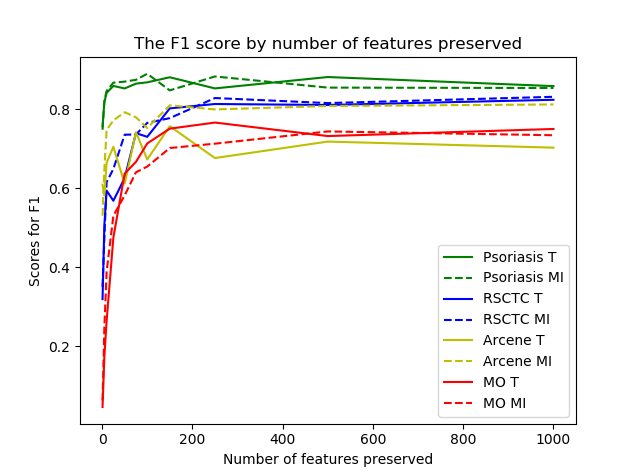
\includegraphics[width=0.7\textwidth]{Data_Rank_F1_Scores.png}
		\caption{The average validation F1-scores shown per dataset and rank.}
		\label{fig:DatasetRankF1Scores}
	\end{figure}
	
	\subsection{Feature Selection Algorithms Evaluation Results}
	\label{FSsubsec:FeatureSelectionAlgorithmsEvaluationResults}
	
	% Figures + first observations
	The figure showed that all wrapper algorithms preserved on average less than 61 features for these settings, whereas the performance seems to average around 75\%. The filter and embedded methods performed worse, with an overall lower performance score than the wrapper methods, even when more features were present. Also, no immediate observations can be made by looking only at the filter and embedded algorithms.
	
	% Wrapper algorithms observations
	When only looking at the wrapper algorithms, some other observations could be done, as well. Ordering the features before using a wrapper method structurally gave a better result than using a random ordering. Also a threshold of $\alpha = 0.001$ usually resulted in more features and in a higher scores in comparison with a threshold of $\alpha = 0.01$. Comparing the algorithms, the floating search with ordering did best in performance, whereas the other algorithms are performing closer together.

	% Insert figures
	\begin{figure}[H]
		\centering
		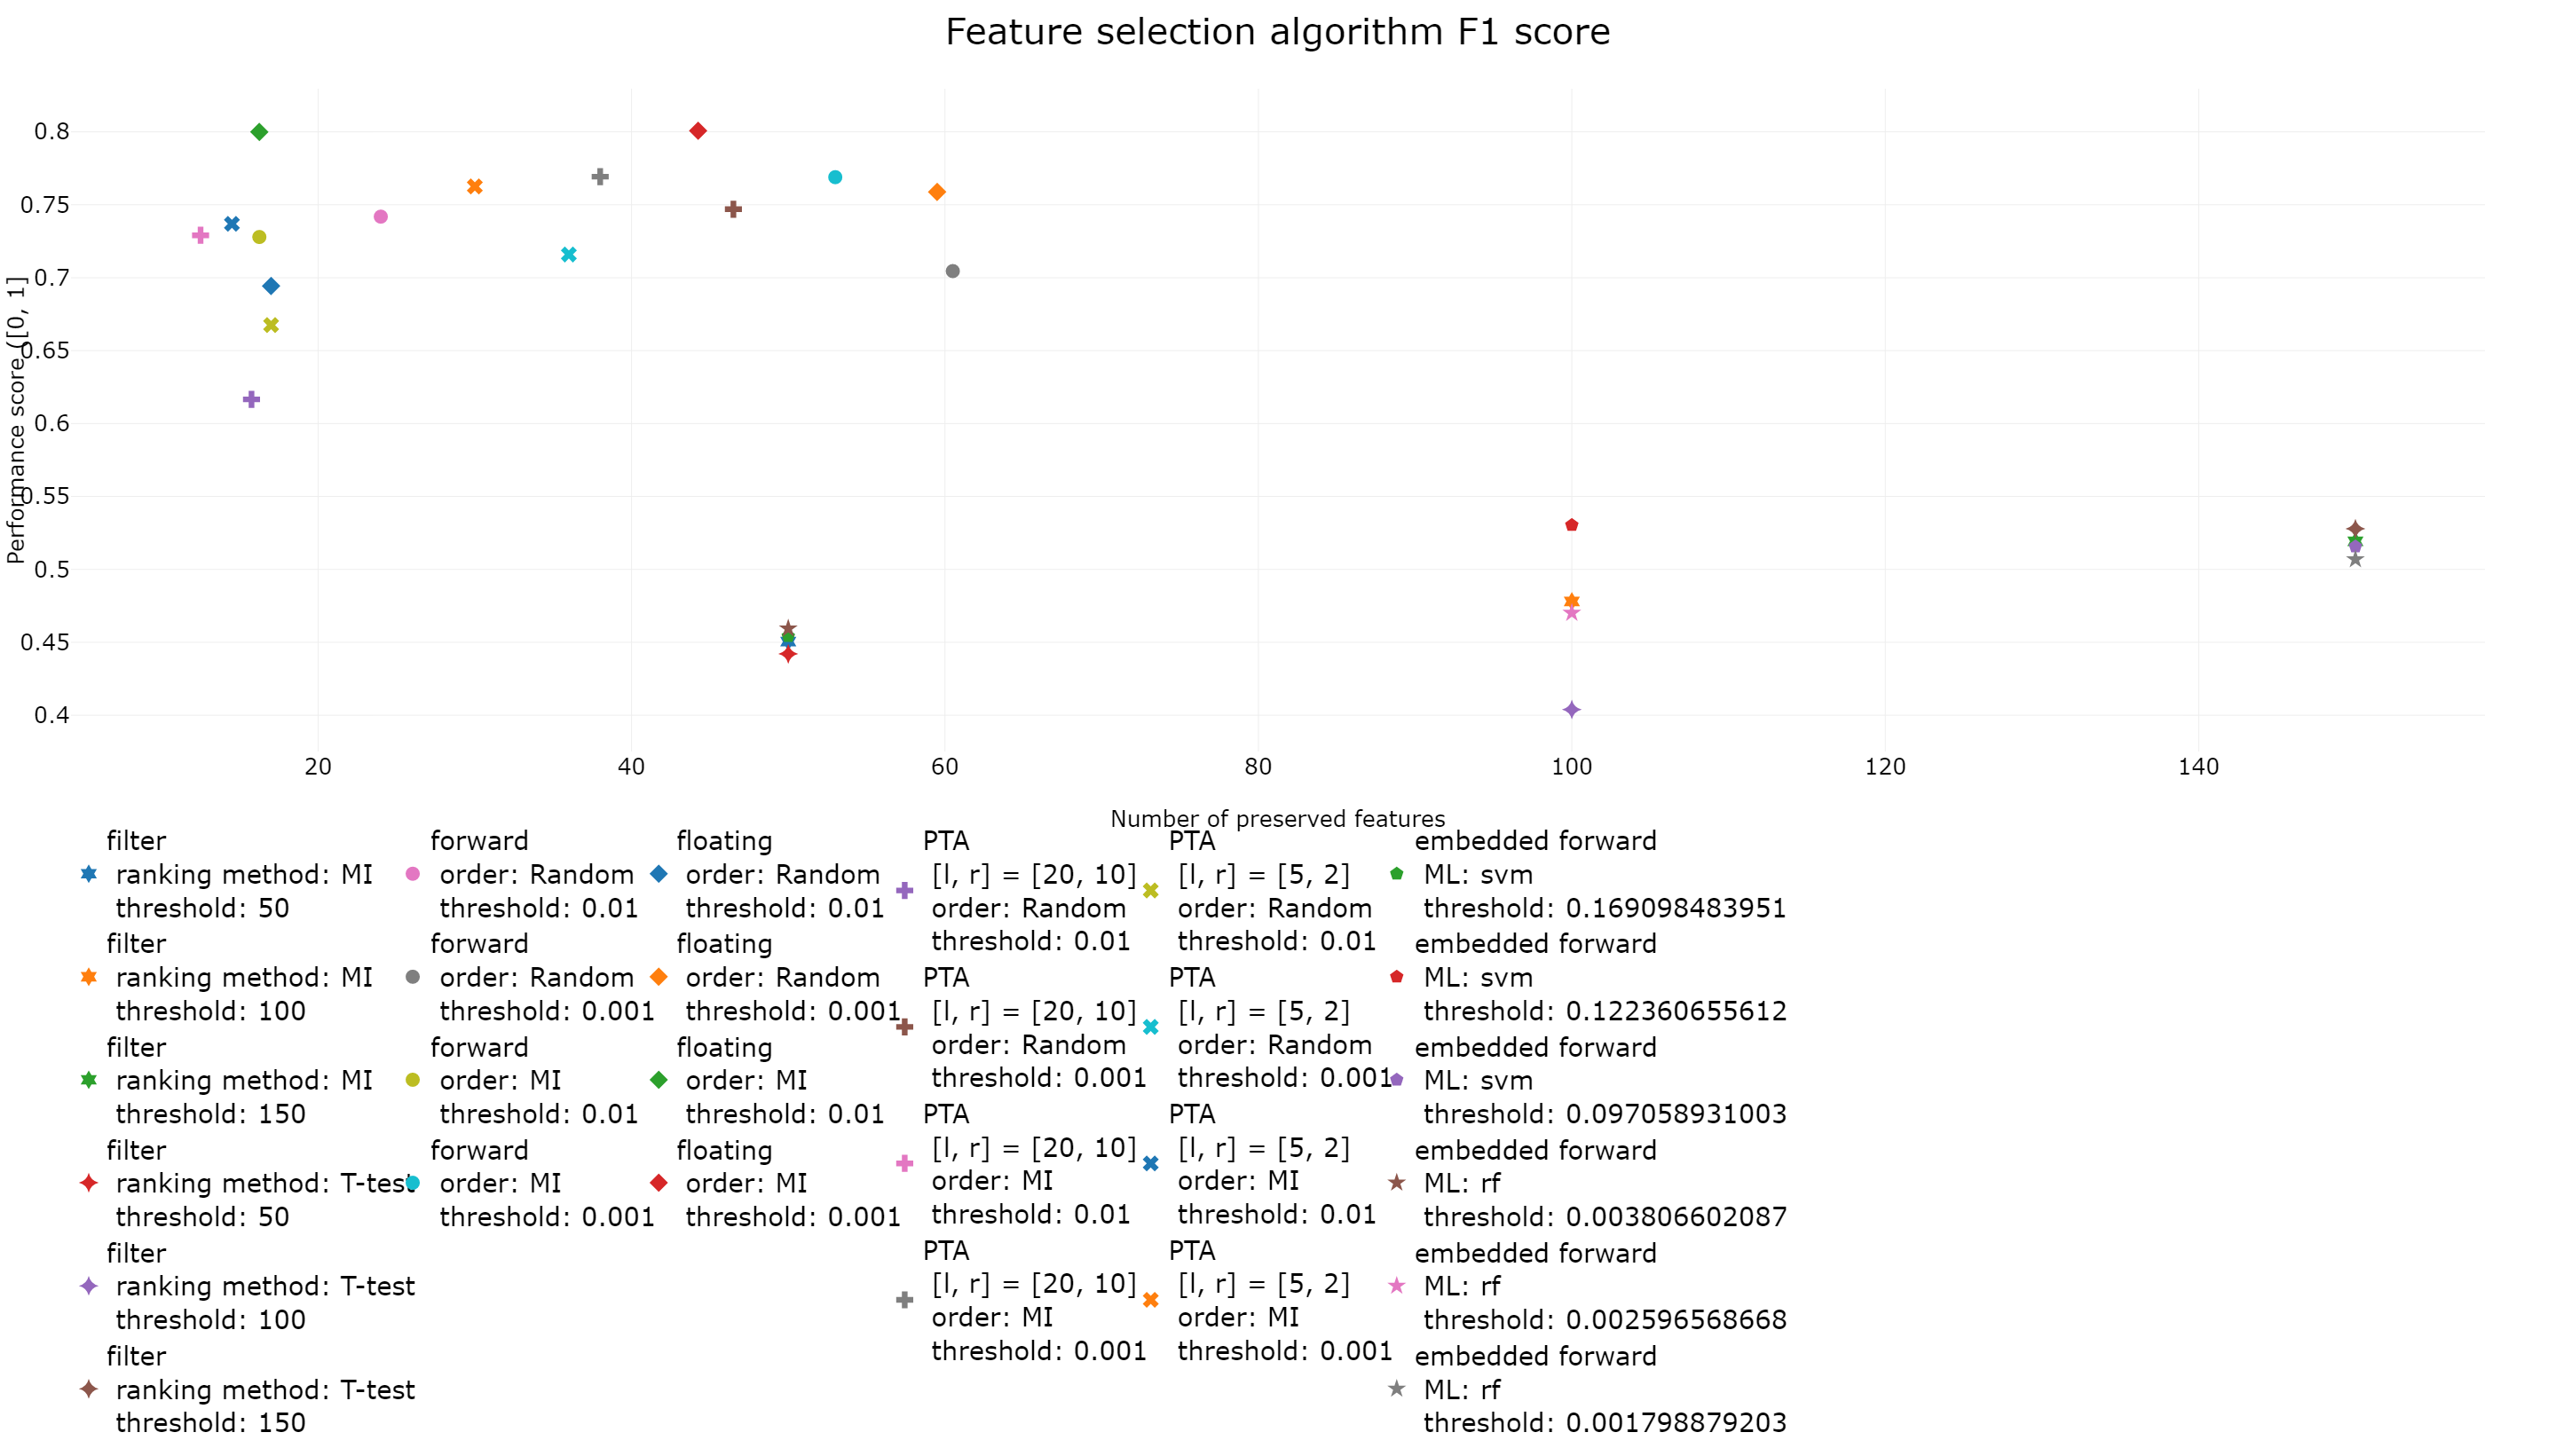
\includegraphics[angle=90,height=1.4\textwidth]{F1_new.png}
		\caption{The F1 spectrum for the average dataset. The x-axis shows the average number of features that are preserved and the y-axis shows the F1 score of logistic regression. The legend indicates the algorithms and their corresponding shapes, as well as the chosen parameters with their matching colours. Abbreviations in legend: Mutual Information (MI), Pick l-Take Away r (PTA), Machine Learning algorithm (ML), Support Vector Machine (svm), random forest (rf)}
		\label{fig:Avg_F1_Spectrum}
	\end{figure}
	
	\subsection{TPOT Feature Selection Integration Results}
	
	To visualize the results of the experiment, a table with the final results is made (Table \ref{tab:TPOTResults}). The optimization process is also recorded and shown in a plot for the four datasets (Figure \ref{fig:TPOTResultMO}). The five experiment reruns are averaged to one complete result.
	
	\begin{table}[]
		\caption{The performance of the final pipeline for the different types of \textit{TPOT} and the mentioned dataset. The five reruns are averaged into this one result.}
		\label{tab:TPOTResults}
		\begin{tabular}{ll|ll|ll}
			\multirow{2}{*}{\textbf{Algorithm}} & selection      & \multicolumn{2}{l|}{regular selection}                                                                                                 & \multicolumn{2}{l}{always feature selection}                                               \\ \cline{3-6} 
			& availability   & \begin{tabular}[c]{@{}l@{}}regular\\ algorithms\end{tabular} & \begin{tabular}[c]{@{}l@{}}feature selection\\ algorithms\end{tabular} & regular algorithms & \begin{tabular}[c]{@{}l@{}}feature selection\\ algorithms\end{tabular} \\ \hline
			\multirow{4}{*}{\textbf{Datasets}}  & Micro-organisms & 0.45                                                        & 0.71                                                                  & 0.64               & 0.59                                                                   \\
			& Arcene         & 0.46                                                        & 0.69                                                                  & 0.62               & 0.69                                                                   \\
			& RSCTC          & 0.00                                                       & 0.22                                                                 & 0.17              & 0.44                                                                       \\
			& Psoriasis      & 0.00                                                       & 0.24                                                                 & 0.16                   & 0.54                                                                      
		\end{tabular}
	\end{table}
	
	\begin{figure}[H]
		\centering
		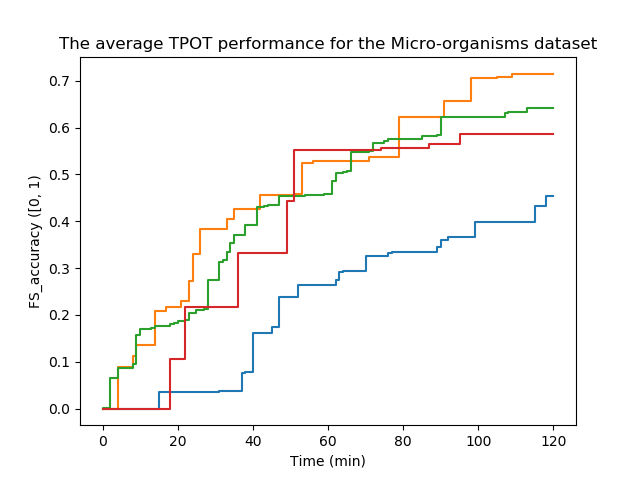
\includegraphics[width=0.8\textwidth]{TPOT_avg_MO.PNG}
		\caption{The optimization process for the different \textit{TPOT} algorithms for the micro-organisms dataset. - \underline{TO DO: Make one for all 4 datasets}}
		\label{fig:TPOTResultMO}
	\end{figure}
	
	% Results \textit{TPOT}
	The results show that after two hours of running \textit{TPOT}, regular \textit{TPOT} always performs worst. According to the processes the high feature selection algorithm set shows much more big stepwise improvements, accompanied with fewer smaller stepwise improvements. This shows the earlier observed trade-off between computation time and feature selection quality for these specific feature selection algorithms. It takes longer to compute those algorithms, but it also gives a much better result. 
	
	% Best \textit{TPOT} type
	The choice for the best \textit{TPOT} algorithm is not conclusive. For high feature selection, all three new possibilities show improved results. The \textit{TPOT} variant that is feature selection focused and has the new feature selection algorithm set performs the best for datasets with a very high number of features (RSCTC and Psoriasis), but the trade-off in computation time seems to hurt the performance for smaller datasets. The algorithm that is only feature selection focused has a steady performance for datasets with a lower number of features, but this performance does not seem to be better than the algorithm with only the new feature selection algorithm set.

	\section{Discussion}
	\label{FSsec:Discussion}
	
	% Research relevance
	There are several works focused on the possibility of feature selection, both with a data analytical \cite{catal2009investigating} as well as a biomedical \cite{baumgartner2006data, welthagen2005comprehensive, liu2002comparative} point of view. These research projects are usually focused on datasets with a low number of features, for which feature selection is less relevant. This research for datasets that have a significantly higher number of at least 1000 features is new, even though newly available datasets become bigger over time due to new and improved techniques of measuring and storing data. With this research a beginning is made on how to approach feature selection on these bigger datasets.
	
	% Wrapper methods exclusion
	Whereas multiple feature selection methods are discussed, several were not tested due to computation time constraints. The wrapper methods backwards elimination and simulated annealing and the embedded backwards elimination all were too computationally intensive to become relevant for the research. In datasets with fewer features, these methods may be showing better results and could be possible candidates for feature selection.
	
		% Filter method exploration
	After evaluation of the results in the first experiment set-up, it could be concluded that there was not a big difference between using T-test/ANOVA or Mutual Information as a ranking method. Both gave similar results, with the exception of one dataset. 
	
	% Second conclusion exploration
	A second conclusion was drawn from looking at the accuracy with the number of features preserved. After a threshold of 200 features, additional features did not raise the validation score as much as the first 200 features did. This indicated a second rule of thumb, that at least 200 features should be preserved after using a filter method. This rule of thumb was according to the hypothesis H1 notion that at most 1000 features should be preserved to still show an efficient result, however was much lower than the expected upper bound of 1000 features. This absolute number was not intuitive and much lower than expected. More research could be done on these preserved 200 features and why no other features were needed to predict the output. Cluster analyses for example may show insights in this phenomenon.
	
	% Second experiment - filter vs wrapper methods
	After evaluation of both filter, wrapper and embedded methods, wrapper methods were significantly better at selecting a smaller fraction of features while preserving a similar test score.  Whereas hypothesis H2 stated wrapper methods to be best in efficiency, embedded methods were expected to outperform both filter methods and wrapper methods when looking at both quality and computation time. This was not the case, however, as embedded methods had a near identical quality to filter methods and performed much worse than wrapper methods. The outcome indicated that wrapper methods are significantly different in results and filter and embedded methods being nearly identical.
	
	% Further conclusions
	Since wrapper methods take dependencies between features into account, they kept these dependencies at a minimum. If these dependencies are unwanted, wrapper methods are more useful than filter methods and embedded and should be recommended. A downside of the wrapper methods however was that they took much more computation time than the filter and embedded methods. Therefore if it does not matter when features have dependencies with each other, a filter method should be recommended.
	
	% Wrapper methods with each other
	There was a difference in quality within the wrapper methods. The forward selection and PTA all showed promising results and therefore should be considered for the framework. Floating search showed the best results, however took significantly longer in computation time. Within the wrapper methods, an ordering beforehand showed improved results. Backward elimination wrapper algorithms, stochastic search algorithms and embedded backwards elimination algorithms all were significantly worse in computation time than the other wrapper algorithms and therefore should not be considered in these cases.
	
	% Threshold wrapper methods
	A recommendation for the threshold in wrapper methods is not trivial. A higher threshold of $\alpha = 0.01$ gave a smaller feature subset at the cost of a lower classification score. If a smaller subset is desired or more influential features are needed, a bigger threshold should be chosen, whereas it will be smaller when a higher quality of the feature subset is desired.
	
	% \textit{TPOT} conclusion
	Both additions to \textit{TPOT} were beneficial according to the experiment. This was also expected, as H3 states.  When the initial number of features was very high (50.000), a combination of initial bias towards feature selection and using feature selection algorithms focusing on preservation of only 200 features performed best. For lower number of features only adding one of the improvements was better, as computation time became the limiting factor in case of using both improvements.
	
	\bibliography{../References/Citings} 
	\bibliographystyle{ieeetr}
	
\end{document}
